\chapter{State of the Art} \label{chap:State of the Art}

\section{Implementation of Reactive Systems}

	\subsection{Observer Design Pattern}

	\subsection{Reactive Programming}

	\subsection{RxJs and BaconJs}

	\subsection{Debugging Reactive Code}
	% other systems that do


\section{Previous and Related Work}
	\subsection{The Chrome Reactive Inspector}
		% everything done by my predecessors in short, focus of both works and what differed
		\subsubsection{Master Thesis by Waqas Abbas}
		\subsubsection{Master Thesis by Pradeep Baradur}
		\subsubsection{Merging previous efforts}
		%...
		\subsubsection{"Special Curicumstances"}
		% demo version of jalangi
		% instrumenting files via scanning the html for script tags
		% -> will not work for module loaders like require.js or ecma6
		% -> will not work with bundled javascript code - but since in development there should be a non bundled version available not 
		% a big problem in javascript. But for Typescript since the extension does not support it and when compiling there may already be bundling in place. (#add some text from future here#)
	% shared context through "new Function" that breaks the separation enforced by chrome (previous code eval)	
	

	\subsection{RxFiddle}
	% features of RxFiddle
	% limitations: 'one of the limitations of RxFiddle is ... which we tackeld in this work.
	% test rxFiddle with one example that generates thousands of steps


% end of state of the art chapter
%----------------------------------------------------------------------------
%latex sample code:



\begin{figure}[!h]
	\centering
	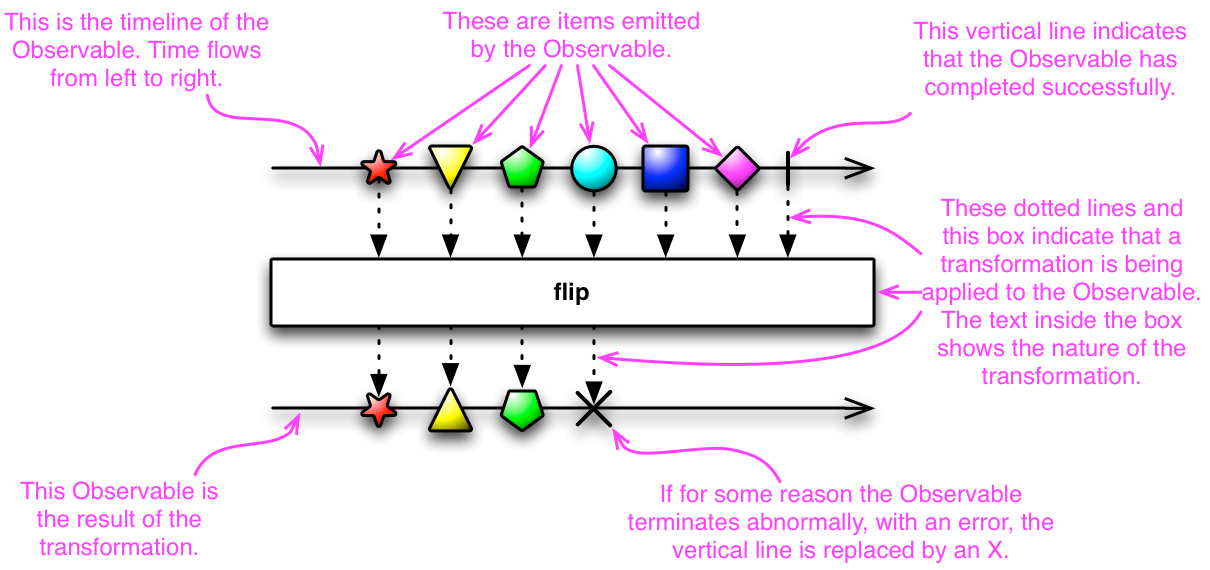
\includegraphics[scale=0.5,trim=0 0 0 0]{gfx/rxjs-reactive-pattern2.png}
	\caption{Reactive pattern \protect\cite{ReactiveXobservable}}
	\label{fig:rxjs-reactive-pattern}
\end{figure}

\textbf{Observable and Observer}\\
Placeholder

\textbf{Operators}
\label{subsec:Operators}\\

\textbf{RxJS Code Structure}\\
Placeholder
\begin{lstlisting}[language=JavaScript, caption=RxJS Simple Example, label={lst:RxJS_Simple_Example}]
// 1. Srouce Observable Creation
var sourceObservable = Rx.Observable.interval(1000);
// 2. Transformation by applying different operators
var transformedObservable = sourceObservable.map(function(x) {
		return x * 10;
	})
	.filter(function(x) {
		return x !== 20
	})
// OUTPUT
Next: 0
Next: 10
Next: 30
Next: 40
Next: 50
Completed
\end{lstlisting}

\subsection{Bacon.js}

\textbf{EventStream and Property}\\
Placeholder

